\section{Process Background}

    \begin{itemize}
        \item tomography - 3d
        \item wigner functions Wigner quasiprobability distribution aka Wigner function - violates Kolmogorov axioms as they have regions of negative probability density
        \item gpd relation
        \item dvpi relation
        \item other measurements
        \item Overview of this measurement
    \end{itemize}
    
    'Tomography' comes from the Greek 'Tomos', meaning to section or slice


    The term 'tomography' is derived from the Greek word 'tomos,' which translates to 'slice' or 'section.' It is a concept extensively applied in the realm of modern medical imaging. For instance, computed tomography (CT), a term many people are familiar with, involves the use of a set of X-rays to generate a three-dimensional reconstruction of bodily organs. This ability to visualize an object's internal structure without disruption opens up a plethora of applications in various fields, from medicine to material science. Building on this concept, 'proton tomography' represents a leap forward into the subatomic scale, harnessing nuclear reactions to reconstruct 3D parton distributions within a nucleon, the core building block of the atomic nucleus. This innovative technology serves as a bridge between the macroscopic world familiar to most, exemplified by CT scans, and the microscopic world of particle physics, providing unprecedented insights into the structure and properties of matter at its most fundamental level.


    
    Discussion of Form Factors and genralized proton structure, Wigner Functions


volker proton pressure \cite{Burkert2018TheProton}

will detmold phialia proton pressure theory \cite{Shanahan2019PressureProton}


From FNPP: 
In understanding the microscopic nature of matter, we rely on two main approaches. One can probe the spatial distribution of matter (charge or current) in a system through elastic scattering of electrons, photons, neutrons, etc. One measures the elastic form factors, which depend on the momentum transfer to the system, and then the Fourier transform of these form factors can provide information on the spatial distribution. Examples are the charge distribution in an atom and the atomic structure of a crystal. An alternative approach is to consider the distribution of constituents in momentum space by measuring deep-inelastic knockout. Examples of this approach include the proton distribution in nuclei measured via quasielastic electron scattering (see Chapter 16) and the distribution of atoms in a quantum liquid studied using neutron scattering. With some modifications to accommodate the relativistic nature of the system, both experimental approaches have been used to explore the interior of the nucleon. The elastic nucleon form factors have been measured with ever-increasing precision since the 1950s and at low momentum transfer (<< nucleon mass) where the nucleon recoil effect is small, the three-dimensional Fourier transform of the form factors is interpretable as the spatial charge and current distributions of quarks. On the other hand, the parton distributions measured in DIS are the longitudinal momentum distributions of the quarks and the gluons in the infinite momentum frame. Both observables have provided great insight into the structure of the nucleon, but both have deficiencies. The form factors contain no dynamical information on the constituents, such as their velocity and angular momentum. The momentum distributions provide no information on the spatial structure. More complete information about the microscopic structure lies in the correlation between momentum and spatial coordinates, i.e., simultaneous knowledge of a constituent's location and velocity. This knowledge is attainable for a classical system, for which one can define and study the phase-space distribution. For a quantum mechanical system, however, the notion of a phase-space distribution seems less useful because of the Heisenberg uncertainty principle: one cannot determine the position and conjugate momentum of a particle simultaneously with arbitrary precision. Nevertheless, the first quantum mechanical phase-space distribution was introduced by Wigner in 1932 and these distributions have been used in a number of areas, e.g., heavy-ion collisions, quantum molecular dynamics, signal analysis, etc.

The notion of a correlated parton position-and-momentum distribution had not been systematically explored in QCD until a few years ago. The generalized parton distribution (GPD) is a one-body matrix element that combines the kinematics of both elastic form factors and parton distributions, and is measurable in hard exclusive processes. GPDs were introduced as objects with interesting perturbative QCD evolution, but were largely ignored because of unclear physical significance. They were rediscovered in the study of quark orbital motion and the spin structure of the nucleon in which the physics potential of the distributions began to surface.

The quest to experimentally determine the GPDs has focused on deep-inelastic exclusive production of photons, mesons and lepton pairs. We consider briefly two experiments that have been extensively studied: deeply virtual Compton scattering (DVCS), in which a real photon is produced, and diffractive meson production. DVCS is cleaner, but the cross section is reduced by a factor of $1/\alpha$; meson production is easier to detect, but it is suppressed by factors of $1/Q^2$.

As nucleon matrix elements, GPDs must be calculable in the fundamental theory. At present, our only way to compute, rather than model, QCD dynamics is lattice field theory. The physical significance of GPDs was first revealed in studying the spin structure of the nucleon. One can decompose the nucleon's spin as:



\begin{equation}
\frac{1}{2} = J_q(\mu) + J_g(\mu)
\end{equation}

where the $J_{q,g}$ are the contributions from the quarks and gluons, respectively. Both contributions are gauge-invariant but renormalization scale-dependent. The $J_{q,g}$ can be expressed as matrix elements of the QCD energy-momentum tensor $T_{\mu \nu}^{q,g}$.

\begin{equation}
J_{q,g}(\mu) = \langle P1/2 \left| \int dx(x \times T_{q,g})_z \right| P1/2 \rangle
\end{equation}



which can be extracted from the form factors of the quark and gluon parts of the $T_{\mu \nu}^{q,g}$. Taking the forward limit of the $\xi = 0$ component and integrating over $x$, one finds that the $A_{q,g}(0)$ give the momentum fraction of the nucleon carried by the quarks and gluons, respectively, i.e., [$A_q(0) + A_g(0) = 1$]. On the other hand, one finds that [Ji97]



\begin{equation}
J_{q,g}(\mu) = \frac{1}{2}[A_{q,g}(0) + B_{q,g}(0)]
\end{equation}


The matrix elements of the energy-momentum tensor provide the fractions of the nucleon spin carried by the quarks and gluons. Because the quark and gluon energy-momentum tensors are examples of twist-two, spin-two, helicity-independent operators, we immediately have the following sum rule for the GPDs

\begin{equation}
    \int \frac{d}{dx}[H_{q}(x, \tau, t) + E_{q}(x, \tau, t)] = A_{q}(t) + B_{q}(t)
\end{equation}

where the $\delta$ dependence is eliminated. If we extrapolate the sum rule to $t = 0$, the total quark contribution to the nucleon spin is obtained. The total quark contribution $J_q$ can be decomposed gauge invariantly into the quark spin $1/2\Delta\Sigma$ and the orbital contribution $L_q$. Extracting $J_q$ from knowledge of the GPDs and $\Delta\Sigma$, the quark orbital angular momentum can be determined. In this way, GPDs offer the potential to provide new insight into the spin structure of the nucleon.

In conclusion, it is important to place the discussion here in the context of a broader theoretical framework. Partons inside the proton can be described by Wigner distributions in six-dimensions (three position and three momentum coordinates). Wigner distributions are the quantum-mechanical constructions that are closest to a classical probability density in phase-space. However, they are not positive definite and are termed quasi-probability distributions. They can be used to compute the expectation value of physical observables. Thus, they represent the maximal knowledge of the partonic structure. They are equivalent to knowing the complete wavefunction of partons inside the nucleon. The distribution $W(x, b_T, k_T)$ is the master Wigner distribution. Here, $b_T$ is the transverse position inside the nucleon and $k_T$ is the transverse momentum of the partons inside the nucleon. By integrating over the transverse position, one is left with transverse momentum distributions (TMDs), while by integrating over transverse momentum, one obtains impact parameter distributions, whose Fourier transform yields the GPDs. The regular parton densities discussed above as well as form factors are derived by subsequent integration.

This modern, theoretical perspective has motivated an experimental program to image the three-dimensional structure of the proton using TMDs, GPDs, PDFs and form factors. Tomography of the nucleon is a major research thrust at the upgraded Jefferson Laboratory as well as a strong motivator for a future electron-ion collider.



Transversity GPDs = helicity flip = chiral odd
helicity conserving = chiral even GPDs, no T subscript. 

From \cite{Amaldi1979Pion-electroproduction}, Gaama is of electromagnetic origin and contains the effect of the electron-photon vertex and the photon propagator. It can be interpreted as the number of virtual photons per scattered electron 

Epsilon can be interpreted as the ratio of transverse to longitudinally polarized photons


Twist-2 and twist operaator expansion


attempt to understand pion production \cite{Goloskokov2010AnElectroproduction}
Burkardt's 2007 work investigates Generalized Parton Distributions (GPDs) \cite{Burkardt2007GPDs0}.
Jaffe deep physics \cite{Jaffe2022DeepPhysics} 
Lee's design of beams is discussed in detail \cite{Lee2019DesignBeam}.
Goloskokov's 2011 work delves into transversity of mesons \cite{Goloskokov2011TransversityMesons}.
Ji discusses gauge-invariant spin in his 1997 study \cite{Ji1997Gauge-InvariantSpin}.
Epstein's 2020 work delves into measurements at the MeV scale \cite{Epstein2020MeasurementMeV}.


Short explanation regarding the connection between “t” dependence and impact parameter.
section 2.3.2 (page 19).


    Now discussion of DVEP:
GPDs, Wigner functions
relationships all the way around
some annoying math
Handbag diagram
Lepton hadron plane
Status of experiments and future (EIC mapping)

        As we increase the resolution (resolve features over smaller spatial distances), what we see is dependent on what resolution scale we are at. An exception to this case is if we are investigating point-like particles, which would have an identical response across all resolution scales


Deep exclusive processes can allow access to Generalized Parton Distributions (GPDs),
a concept that lies at the root of 3D imaging of the proton’s quark-gluon substructure,
as GPDs contain information about the transverse spatial distribution of quarks and their
longitudinal momentum inside hadrons. The key to extracting GPDs from experiments are
the Quantum Chromodynamics (QCD) factorization theorems. Deeply Virtual Compton
Scattering (DVCS) is the cleanest way to
study GPDs. While DVCS data have given hints of the factorization regime being
attained, such hints have not been observed for Deeply Virtual Meson Production (DVMP)
data. Exclusive $\pi^0$ electroproduction has been measured by experiment E12-06-114 in Hall
A of JLab in order to test factorization in DVMP processes. Cross sections have been
measured at three fixed Bjorken- x (xB) : 0.36, 0.48 and 0.6 in the Q2 range 3 to 9 GeV2.
High statistical measurements of polarized and unpolarized cross sections of H(e,e’,gamms)
p could allow mapping and extraction of GPD information from the nucleon. In this talk,
I will show the experimental setup, calibration and preliminary results of the neutral pion
electroproduction cross sections for xB 0.3 from this experiment


Intuition about DVMP
First, note that not all DVMP reactions are sensitive to nuclear transversity distributions,
which involves quark helicity flip of transversely polarized quarks helicity This can occur
in production of pseudoscaler mesons, e.g. pi0 and eta production, with spin-charge-parity
I-PC= 0 - + ,in contrast with the incident photon, which has J-P 1- -. This is not the case
for other mesons studied at JLab, such as vector mesons, I-PC= 0 - e.g. the rho, omega, phi,
for which which I-CP= 1- -, the same as for the photons. I believe this was first pointed out
Ahmad, Goldstein, Liutti (arXiv:0805.3568). Here is a quote from their intro. ”... deeply
virtual $\pi^0$ (as well as$\eta$,$\eta$') production off a proton target is clearly distinct from the other
types of meson production processes in that it involves the transition of a (virtual) photon
with JPC = 1– to a JPC = 0-+ state (i.e. the final $\pi^0$ or$\eta$,$\eta$’) requiring odd C-parity and
chiral odd t-channel quantum numbers. As a consequence, in a partonic description such
as the one depicted in Fig.1a, the ”outgoing” and ”returning” quark helicities need to be
opposite to one another . . . ”.
Peter Kroll, who works very closely this group, with Sergei Goloskokov, Marcus Diehl,
et al. have published extensive theoretical calculations based on Jlab data. Gary Goldstein,
Simonetta Liutti have have also published on this reaction.
By the way, the other meson production channels are uniquely sensitive to other inter-
esting aspects of nucleon structure. For example, the phi, on which F-X and Patrick are
working, is very sensitive to the gluon distribution in the nucleon.
In DVCS the incident and outgoing particles are both photons JP= 1-. Therefore, no
quark helicity flip is necessary in this “virtual Compton scattering”. Therefore DVCS is
primarily sensitive to non-quark spin flip - eg. H.. The same is true with DVMP of other
vector meson, such as rho. However, since the pi0 and eta are JP=0-, then the transverse
photon part contributing to the overall reaction cross section can cause a transversely po-
larized quark helicity flip. This is contained mainly in the structure functions $\sigma$T and $\sigma$T T ,
which can be decomposed into the transverity GPDs - mainly EbarT and HT

Also, pion and eta production can still also be accompanied by non-quark helicity flips,
which would be mainly contained in the longitudinal structure functions $\sigma$LL. However,
various theoretical papers indicate that in our accessible region of Q2, $\sigma$T and $\sigma$T T dominate
relative to $\sigma$L. Experimentally, this seems to be verified from JLab data . On the other
hand, theory predicts that asymptotically, $\sigma$L will dominate. From our existing 5 GeV data,
we are not anywhere near there, so our experiments at JLab are really just right for accessing
these transversity distributions. But, to decompose these distributions at the level of the
individual quark u d flavors, we need as much precision data over as big a range as possible
of kinematics in several channels - P-pi0, N-pi0, P-eta, N-eta. And, only you guys can do
that! So, let me know if this makes sense to you. s a bit.

What do we want at the end of the day and why?
What is the Hall A DVMP measurement? gravitational form factor of the proton Why is
CLAS12 particularly suited for this measurement Compare to other experiemnts - hall A,
compass, etc. Precision estimate – 10\%? 5\% if we are lucky? What was precision of CLAS6?
other note – intution for process – not just getting longitudinal momentum information as
with DIS, but also get the other piece of information from having put back together the
proton. Read about Compton Form Factors/ extensions of. of all electrons that enter target,
how many colissions do we get? probably either 1 or none? what is the probability of 1?
Very important and good stating place - write up notes from 2011 pi0 analysis note
Write to Axel at BIn Volume correction, page 75 analysis note fig 6.1
Compare integrated luminosity of CLAS6 to CLAS12 (in 2011 analysis note)
$\pi^0$ $\rightarrow$ $\gamma$$\gamma$ branching ratio = 98.8\%
Given we have an interaction, how many do we detect (ep)?
Question: WHy is beam charge important? Answer (Brandon Clary, email) The accu-
mulated beam charge is charge measured at the Faraday cup. It’s important for determining
the luminosity for a run, and even being able to compare data from run to run, especially
when runs may have different beam current, for example. It’s just a good way to normalize
to the total number of electron in that run, file, etc. In principle you could normalize by
minutes, hours, etc. But beam charge, number of el., is needed to calculate the luminosity
for a fixed target experiment when extracting cross sections.
263

Low t-data are very important for the meson exclusive physics. The GPD interpretation
works only in the region -t/Q2¡1. From this point of view the central detector will not only
increase the total statistics by a factor more than 2 but will add the valuable data with low
t.
However, for pi0 the only data we have from Hall A are of very limited statistics and
kinematics. One of their limitations was the relatively modest variation on polarization
parameter (epsilon) since the beam energies we not so far apart.
Number of final events in CLAS6 DVMP? About 100K, maybe 200K.
Dear Valery
CLAS12 acceptances and resolutions are also superior to that of CLAS6. Main differences
are: - RGK has outbending torus vs inbending CLAS6 data - the distance between the target
and the PCal has increased, the FTCal extends to lower angles, and the gap between FTCal
and PCal is much smaller than between IC and EC - proton polar angle was limited to 60
deg in the e1dvcs dataset if my memory is correct
Do you have on hands the number of exclusive pi0 events published for the CLAS6
cross-sections? We need numbers to make the case to cook the RGK data
Well over an order of magnitude more statistics at CLAS12 compared to CLAS6


There are 4 *twist-2* quark GPDs for heliicty conserving processes, and 4 for helicity flipping processes. Some questions:
The 8 GPDs are divided into: 4 with subscript T and 4 without. This notation is mostly clear, as T stands for transversity and refers to helicitiy flipping.  4 called "H" and 4 called "E".  4 with a "~" and 4 without. 








THE GPDs H and E are independent of quark helicity and are therefore called unpolarized GPDs whereas Htilde and Etilde are dependent of the quark helicity and are called polarized GPDs

H and Htilde conserve proton spin, while E and Etilde flip the proton spin (overall helicity is not conserved - the proton changes helicity but the quarks do not) 

Modified from DVCS Guegan Thesis


\begin{tikzpicture}
    \begin{feynman}
        \vertex (i1) {$e^{-}$};
        \vertex[right=1cm of i1] (v1);
        \vertex[below=2cm of i1] (i2) {$p$};
        \vertex[right=1cm of i2] (v2);
        \vertex[right=2cm of v1] (o1) {$e^{-}$};
        \vertex[right=2cm of v2] (o2) {$p$};
        \vertex[above right=1cm and 1cm of v2] (v3);
        \vertex[right=1cm of v3] (o3) {$\bar{q}$};
        \vertex[below right=1cm and 1cm of v3] (o4) {$q$};

        \diagram* {
            (i1) -- [fermion] (v1) -- [fermion] (o1),
            (i2) -- [fermion] (v2) -- [fermion] (o2),
            (v1) -- [photon, edge label=$\gamma^{*}$] (v2),
            (v2) -- [fermion] (v3),
            (v3) -- [fermion] (o3),
            (v3) -- [anti fermion] (o4),
        };
    \end{feynman}
\end{tikzpicture}

%Deeply (Q2 >> M^2) Inelastic (W2 >>M2) Scattering



\subsection{Generalized Parton Distributions}\label{sec:ch1sec2GPDs}

H = quark polarization same as nucleon
E = quark polarization different than nucleon


    There are 8 GPDs, 4 correspond to helicity conserving (chiral even) processes and 4 correspond to helicity flipping (chiral odd) processes: \GPDH,  \GPDE,  \GPDHtilde,  and \GPDEtilde  \quad for chiral even, and \GPDHT,  \GPDET,  \GPDHTtilde, and \GPDETtilde \quad (\GPDETbar = 2*\GPDHTtilde+\GPDET is commonly used)
    
        %\textcolor{red}{    Why do the scrtucture combine in the way they do with the coefficents of cos phi terms and epsilons? - insert old links from papers from 1980s}
        
        \begin{table}[H]
            
            \centering
            \begin{tabular}{@{} *{4}{c} @{}}
                    \headercell{Nucleon \\ Polarization} & \multicolumn{3}{c@{}}{Quark Polarization}\\
                    \cmidrule(l){2-4}
                    & U & \textcolor{white}{lllll}L & T    \\ 
                    \midrule
                      U  & \GPDH &               *                    &  \GPDETbar = 2*\GPDHTtilde+\GPDET  \\
                      L  &    *                &  \textcolor{white}{llll}\GPDHtilde &     \GPDETtilde?                              \\
                      T  & \GPDE &               \GPDEtilde ?                    &  \GPDHT,\GPDHTtilde \\
                \end{tabular}\\
    
                \label{GPDsPolarization}
                \caption[GPDs Across Nucleon and Quark Polarizations.]{GPDs Across Nucleon and Quark Polarizations.  * forbidden by parity.}
        \end{table}

          The cross-section for DV$\pi^0$P \eqref{eq:DVPiPCrossSection_theory} can be theoretically linked in terms of structure functions to GPDs, which describe the 3D structure of the nucleon.

    
     \begin{equation}\labelAndRemember{eq:DVPiPCrossSection_theory}
           {\frac{d^4\sigma_{ep \rightarrow ep'\pi^0}}{dQ^2dx_Bdtd\phi_{\pi}} =
         \Gamma (Q^2, x_B, E)
         \frac{1}{2\pi}
         \left\{ \left(  \textcolor{sigmaT}{\frac{d\sigma_T}{dt}}+\epsilon  \textcolor{sigmaL}{\frac{d\sigma_L}{dt}} \right)+
         \epsilon cos(2\phi)  \textcolor{sigmaTT}{\frac{d\sigma_{TT}}{dt}} + 
         \sqrt{2\epsilon(1+\epsilon)} cos(\phi)  \textcolor{sigmaLT}{\frac{d\sigma_{LT}}{dt}} \right\}}
     \end{equation}      \myequations{  \quad  DV$\pi$P Cross Section Decomposition}


     Here $\Gamma$ is the virtual photon flux as in \eqref{eq:virtualphotonflux}, $\epsilon$ is the virtual photon polarization \eqref{eq:virtualphotonpolarization}, and the structure functions can be expressed as convolutions of GPDs as shown in \eqref{eq:sigmaL}-\eqref{eq:sigmaTT}

In the end, H and E encloses the d.o.f in Matrix Elements like as Pauli and Dirac FF do. The tilde ones are about axial OPE, which is not trivial at the tree-level EM elastic interaction. 

    \begin{equation}\label{eq:virtualphotonflux}
                 \Gamma (Q^2, x_B, E) = \frac{\alpha}{8\pi} \frac{Q^2}{m^2_pE^2}\frac{1-x_B}{x_B^3}\frac{1}{1-\epsilon}
    \end{equation}\myequations{Virtual Photon Flux}

    \begin{equation}\label{eq:virtualphotonpolarization}
        \epsilon = \frac{1 - y - \frac{Q^2}{4E^2}}{1 - y + \frac{y^2}{2} + \frac{Q^2}{4E^2}}
    \end{equation}\label{Virtual Photon Polarization}

 \begin{equation}\label{eq:sigmaL}
         \textcolor{sigmaL}{\frac{d\sigma_{L}}{dt}} = 
        \frac{4\pi\alpha}{kQ^2}\left\{ \left( 1 - \xi^2 \right) 
        \lvert \langle \GPDHtildeEQ \rangle \rvert ^2 
        -2\xi^2 \Re \left[  \langle \GPDHtildeEQ \rangle ^* \langle \GPDEtildeEQ \rangle    \right] - \frac{t'}{4m^2}\xi^2
        \lvert \langle \GPDEtildeEQ \rangle \rvert ^2  \right\}
    \end{equation} 

    \begin{equation}\label{eq:sigmaT}
        \textcolor{sigmaT}{\frac{d\sigma_{T}}{dt}} = 
        \frac{2\pi\alpha \mu_{\pi}^2}{kQ^4}
        \left\{ \left( 1 - \xi^2 \right) 
        \lvert \langle \GPDHTEQ \rangle \rvert ^2
        - \frac{t'}{8m^2}
        \lvert \langle \GPDETbarEQ \rangle \rvert ^2  \right\}    
    \end{equation} 
    
    \begin{equation}\label{eq:sigmaLT}
        \textcolor{sigmaLT}{\frac{d\sigma_{LT}}{dt}} = 
        \frac{4\pi\alpha \mu_{\pi}}{\sqrt{2}kQ^3}
        \xi\sqrt{1-\xi^2}
        \frac{\sqrt{-t'}}{2m}
        \Re \left\{ 
         \langle \GPDHTEQ \rangle ^*
        \langle \GPDEtildeEQ \rangle   
        \right\}
     \end{equation} 
    
    
    \begin{equation}\label{eq:sigmaTT}
        \textcolor{sigmaTT}{\frac{d\sigma_{TT}}{dt}} = 
        \frac{4\pi\alpha \mu_{\pi}^2}{kQ^4}
        \frac{-t'}{16m^2}
        \langle \GPDETbarEQ \rangle^2   
    \end{equation} 



    
    The terms involved in these expressions are:
   
    \begin{itemize}
    \item t' = t - $t_0$ where $t_0 = \frac{-4m^2\xi^2}{1-\xi^2}$
    \item Skewness $\xi = \frac{x_B}{2-x_B}$
    \item   The bracket $\langle \tilde{F} \rangle$ is the convolution of a GPD and an appropriate subprocess amplitude:
    $
    \langle \tilde{F} \rangle =  \Sigma_{\lambda} \int_{-1}^{1} d\bar{x}H_{0\lambda,0\lambda}\left( \bar{x}, \xi, Q^2, t=0  \right)\tilde{F}\left( \bar{x}, \xi, Q^2, t  \right)\  
    $
    \begin{itemize}
        \item $\lambda$ is the unobserved helicites of the partons participating in the subprocess 
    \end{itemize}
    \item Phase space factor \scalebox{1}{%
     $           k = 16\pi \left( W^2 -m^2)\sqrt{\Lambda(W^2,-Q^2,m^2)} \right)$ 
    }
    \begin{itemize}
    \item $\Lambda(W^2,-Q^2,m^2)$ is the Källén function: $W^4 + Q^4 + m^4 + 2W^2Q^2 + 2Q^2m^2 - 2W^2m^2$
    \end{itemize}
    
    \item Reduced pion mass     \scalebox{1}{%
      $         \mu_{\pi^0} = \frac{m^2_{\pi^0}}{m_u+m_d}$ 
    }
    \begin{itemize}
        \item   $m_u$ and $m_d$ are respective masses of up and down quarks
    \end{itemize}
    \end{itemize}

K\"{a}ll\'{e}n function,
    
    
    
    

  


    
    
    
    


    

        Include proton pressure distribution plot

      


In addition to collinear momentum distribution of partons inside the
nucleon, GPDs also encode the distribution of partons in the plane transverse to
the nucleons momentum in the infinite momentum frame [58]. Moreover, their
relation to energy-momentum tensor (EMT) form factors allow us to access the
EMT densities, the distribution of energy, angular momentum, pressure, and shear
forces inside the nucleon [15].

Only valence quarks contribute electroproduction of uncharged pions.


    \subsection{Deeply Virtual Exclusive Processes}

\subsection{Deeply Virtual Neutral Pion Production}


 DVMP is sensitive to chiral odd GPDs, distinguishing it from DVCS as a GDP probe because why? Because something involving photon helicity and pion helicity, I forget exactly though


    \subsection{Overview of Experimental Status}
     - Prevous measurements
     Hall A Rosenbluth separation \cite{Defurne2016RosenbluthSection}

     
     - Scope of this analysis
    





\iffalse
        The following is from a paper on pi+ production. This formula is equvalent to the normal convetion (not using W as a variable)
        
         \begin{equation}\label{xsec}
             \frac{d^4\sigma_{\gamma^*p \rightarrow p'\pi^0}}{dQ^2W^2dtd\phi_{\pi}} =
             \frac{\alpha (W^2-m^2)}{16\pi^2 E^2_L m^2 Q^2 (1-\epsilon)}
             ((\frac{d\sigma_T}{dt}+\epsilon\frac{d\sigma_L}{dt})+
             \epsilon cos(2\phi) \frac{d\sigma_{TT}}{dt} + \sqrt{2\epsilon(1+\epsilon)}cos(\phi)\frac{d\sigma_{LT}}{dt})
        \end{equation}
        
        Comparing the two, we have a difference in the prefactor of:
        
        0.3894 * 1E6 * $\frac{1}{16\pi(W^2-m_p^2)\sqrt{W^4 + (Q^2)^2+m_p^4+2W^2Q^2-2W^2m_p^2+2Q^2m_p^2}}$
        
        This factor is accounted for by the Kallen function phase space term.
        
        
        
        
        t' stands for.. t - $t_0$ where $t_0 = \frac{-4m^2\xi^2}{1-\xi^2}$
        
           Where the skewness parameter is $\xi = \frac{x_B}{2-x_B}$ 
           
        
        
            Where $\lambda$ is the unobserved helicites of the partons participaing in the subprocess
            
         and epsilon is... 
            
            
            
            
         
               
            And k is the phase space factor given as 
             \scalebox{0.7}{%
             $           k = 16\pi \left( W^2 -m^2)\sqrt{\Lambda(W^2,-Q^2,m^2)} \right)$ 
            }
            
                Where $\Lambda(W^2,-Q^2,m^2)$ is the Källén function and $\mu_{pi}$ is the reduced pion mass given as 
               \scalebox{0.7}{%
              $         \mu_{\pi^0} = \frac{m^2_{\pi^0}}{m_u+m_d}$ 
            }
            $m_u$ and $m_d$ are respective masses of up and down quarks.
            
             Where $\Gamma (Q^2, x_B, E)$ is the virtual photon flux, is 
             \scalebox{0.7}{%
                $         \Gamma (Q^2, x_B, E) = \frac{\alpha}{8\pi} \frac{Q^2}{m^2_pE^2}\frac{1-x_B}{x_B^3}\frac{1}{1-\epsilon}$ 
            }

\fi


Several weeks ago I remarked in our meeting that I was having difficulty finding an explanation for the specific form of the DVMP cross section written in terms of structure functions (example below). Papers normally state that the relation holds without justification. I tried to follow the papertrail for the origin but so far have not ultimately been successful. Igor has kindly found a paper from 1992 (Dreschsel and Tiator pdf (iop.org) which makes reference (page 460, eq 18 - 19) \cite{Dreschsel1992ThresholdNucleons}
\cite{Bedlinskiy2014ExclusiveCLAS}


to Donnachie and Shaw (Generalized Vector Dominance 1978) \cite{Donnachie1978GeneralizedDominance}


In the attached, Bill Donnelly and colleagues have recently published a long paper
on the general tensor structure for electron scattering in terms of invariant responses.
In Eq (46), they derive a general expression for the Lorentz invariant part of the spin \cite{Donnelly2023GeneralResponses}
dependent cross section.  The unpolarized piece has the identical L/T/TT/TL form you have.
I have not read the paper in detail but I think you may find it useful.



Origin of form and interpretation of virtual photon flux gamma: \cite{Amaldi1979Pion-electroproduction} page 6


By measuring DVMP, we can get information about GPDs in the following way – in the leading twist approximation / some other formalism bullshit, dvmp cross section is described by the generalized Compton form factors, which themselves are (to leading twist etc.) convolutions of GPDs, so the dvmp cross section sets constraints on GPD behavior.

  hard exclusive pseudoscalar meson electroproduction in recent years has shown that the asymptotic leading twist approximation is not readily applicable in the range of kinematics accessible to current experiments. In fact, there are strong contributions from transversely polarized virtual photons that are asymptotically supprsed by $1/@^w$ in the cross sections and have to be considered by introduing chiral-odd GPDs into the framework.   



Hi Bobby, so sorry for late reply I was busy with readiness review preparation.
So Q2>1 is indeed for deeply virtual events, however it has no relation with lepton/hadron angle. There are pi0 events in the region below 1GeV2, and they are also pi0 events. The limit on 1GeV2 is somewhat artificial. Ideally we are looking at the asymptotic freedom, so Q2 should be infinity, but we are hoping that 1GeV2 is big enough to apply models that are based on asymptotic freedom. There are many terms also that are proportional to powers of t/Q2. So we need reasonably big Q2 to apply GPDs models. And in fact CLAS kinematics is often questioned to be too small for GPDs theoretical models.


    DVMP:

    Deep exclusive processes can allow access to Generalized Parton Distributions (GPDs), a concept that lies at the root of 3D imaging of the proton's quark-gluon substructure, as GPDs contain information about the transverse spatial distribution of quarks and their longitudinal momentum inside hadrons. The key to extracting GPDs from experiments are the Quantum Chromodynamics (QCD) factorization theorems. Deeply Virtual Compton Scattering (DVCS) is the cleanest way to
    
    study GPDs. While DVCS data have given hints of the factorization regime being attained, such hints have not been observed for Deeply Virtual Meson Production (DVMP) data. Exclusive $\pi^0$ electroproduction has been measured by experiment E12-06-114 in Hall A of JLab in order to test factorization in DVMP processes. Cross sections have been measured at three fixed Bjorken- x (xB) : 0.36, 0.48 and 0.6 in the Q2 range 3 to 9 GeV2. High statistical measurements of polarized and unpolarized cross sections of H(e,e',gamms) p could allow mapping and extraction of GPD information from the nucleon. In this talk, I will show the experimental setup, calibration and preliminary results of the neutral pion electroproduction cross sections for xB >0.3 from this experiment.  



        First, note that not all DVMP reactions are sensitive to nuclear transversity distributions, which involves quark helicity flip of transversely polarized quarks helicity  This can occur in  production of pseudoscaler mesons,  e.g. pi0 and eta production, with spin-charge-parity  I-PC= 0 - + ,in contrast with  the incident photon, which  has J-P 1- -. This is not the case for other mesons studied at JLab, such as vector mesons, I-PC= 0 - e.g. the rho, omega, phi, for which which I-CP= 1- -, the same as for the photons.   I believe this was first  pointed out  Ahmad, Goldstein, Liutti (arXiv:0805.3568). Here is a quote from their intro.
        "... deeply virtual $\pi^0$ (as well as $\eta$, $\eta'$) production off a proton target is clearly distinct from the other types of meson production processes in that it involves the transition of a (virtual) photon with JPC = 1-- to a JPC = 0-+ state (i.e. the final $\pi^0$ or $\eta$, $\eta$') requiring odd C-parity and chiral odd t-channel quantum numbers. As a consequence, in a partonic description such as the one depicted in Fig.1a, the ”outgoing” and ”returning” quark helicities need to be opposite to one another …". 
        
        Peter Kroll, who works very closely this group, with Sergei Goloskokov, Marcus Diehl, et al. have published extensive theoretical calculations based on Jlab data.   Gary Goldstein, Simonetta Liutti have have also published on this  reaction.
        
        By the way, the other meson production channels  are uniquely sensitive to other  interesting aspects of nucleon structure. For example, the phi, on which F-X and Patrick are working, is very sensitive to the gluon distribution in the nucleon.
        
        In DVCS the  incident and  outgoing particles are both photons JP= 1-. Therefore, no quark helicity flip is necessary in this “virtual Compton scattering”.  Therefore DVCS is primarily sensitive to non-quark spin flip - eg. H.. The same is true with DVMP of other vector meson, such as rho.  
    	However,  since the pi0 and eta are JP=0-, then the transverse photon part contributing to the overall reaction cross section can cause a transversely polarized  quark helicity flip. This is contained mainly  in the structure functions $\sigma_T$ and $\sigma_{TT}$, which can be decomposed into the transverity GPDs - mainly $Ebar_T$ and $H_T$. 
    	
    	Also, pion and eta production can still also be accompanied by non-quark helicity flips, which would be mainly contained in the longitudinal structure functions $\sigma_{LL}$. However, various theoretical papers indicate that in our accessible region of $Q^2$, $\sigma_T$ and $\sigma_{TT}$ dominate relative to $\sigma_L$. Experimentally, this seems to be verified from JLab data .
    	On the other hand, theory predicts that asymptotically, $\sigma_L$ will dominate. From our existing 5 GeV  data, we are not anywhere near there, so our experiments at JLab are really just right for accessing these transversity distributions.  But, to decompose these distributions  at the level of the individual quark u d flavors, we need as much precision data over as big a range as possible of kinematics in several channels - P-pi0, N-pi0, P-eta, N-eta. And, only you guys can do that!
    	So, let me know if this makes sense to you. s a bit. 
    	
        Why is Phi particularly sensitive to the phi distribution?

        If you look at the proposal you will see the main diagram we are interested in has a pair of gluons from the GPD bag connecting a the hard scattering kernel that comes from the virtual photon fluctuating into a $s\bar{s}$ pair
        
        The process you mention instead has a pair of strange quarks from the GPD bag connecting to the hard scattering kernel directly. 
        
        In practice the two processes happen. From known PDF however the gluon contribution is expected to be significantly larger than the strange quarks contribution. So the intuitive reason would be: the proton has nearly no strangeness but does have a bunch of gluons.
        
        Now it could be that we are wrong and that the proton has more strangeness than what conventional PDF suggest. This could potentially hamper our strategy. However, intrinsic strangeness is in itself a very interesting subject, and if we did come to the conclusion that the proton has more strangeness than is conventionally accepted, then it would be a very important result.
        
        The way I understand why the phi channel probes the gluon GPDs is because the phi meson is a strange-antistrange meson, and so doesn't interact with the up and down quarks that predominantly make up the quark content of the nucleons. This is from the phi cross section proposal: Because of its almost pure $s\bar{s}$ composition $\phi$ production is not affected by scattering from the nucleon’s valence quarks or the light quark sea;
        
        How to probe TMDS?
        About probing TMDs, do you know exactly which groups or what channels can be used to do this at CLAS12? For example, we probe GPDs with DVCS or DVMP. Is there a similar channel that allows access to TMDs?
        
        For first one, look for SIDIS, but I'm not sure about specific channels. I could find slides at
        $https://indico.cern.ch/event/568360/contributions/2487494/attachments/1438684/2213587/PuckettDIS2017.pdf$ from google, but there could be better references. I think I have seen one from collaboration meeting but I'm my way back from Chicago to Boston. You can find whole collaboration meeting slides at $https://www.jlab.org/indico/event/343/other-view?view=standard$



    What is the Hall A DVMP measurement?
    gravitational form factor of the proton
    Why is CLAS12 particularly suited for this measurement
    Compare to other experiemnts - hall A, compass, etc. 
    Precision estimate – 10\%? 5\% if we are lucky? What was precision of CLAS6?
    other note – intution for process – not just getting longitudinal momentum information as with DIS, but also get the other piece of information from having put back together the proton. Read about Compton Form Factors/ extensions of. 
    of all electrons that enter target, how many colissions do we get? probably either 1 or none? what is the probability of 1?
    
    Very important and good stating place - write up notes from 2011 pi0 analysis note
    
    Write to Axel at BIn Volume correction, page 75 analysis note fig 6.1
    
    Compare integrated luminosity of CLAS6 to CLAS12 (in 2011 analysis note)
    
    $pi^0 \longrightarrow \gamma \gamma$ branching ratio = 98.8\%
    
    Given we have an interaction, how many do we detect (ep)?
    
    Question: WHy is beam charge important?
    Answer (Brandon Clary, email) The accumulated beam charge is charge measured at the Faraday cup. It's important for determining the luminosity for a run, and even being able to compare data from run to run, especially when runs may have different beam current, for example. It's just a good way to normalize to the total number of electron in that run, file, etc. In principle you could normalize by minutes, hours, etc. But beam charge, number of el., is needed to calculate the luminosity for a fixed target experiment when extracting cross sections.


    What is event rate? In Hz or in barns. What is your luminosity?
    Diff between Fast MC and GEMC?

            

phi1 = angle(v3l,v3h)
phi2 = angle(v3l,v3g)
where if dot(v31,pro > 0,), phi1 =  360 - phi1
if  dot(v31,pro < 0,), phi1 =  phi1 I think check this

v3l = cross(beam,ele) = pe x pe'
v3h = cross(pro,vgs) = pp' x pgamma*
v3g = cross(vgs,pi0) = pgamma* x ppi0
ppi0 = pgamma1+pgamma2

vgs = (-Epx,-Epy, pbeam-df(EPZ) = (-pe'x, -pe'y, pbeam-pe'z) where pbeam = sqrt(beam-me%^2)

angle = arccos(costheta(vec1,vec2))
costheta = v1*v2/sqrt(v1*v1*v2*v2)

Thus:
phi = arccos( (v3l dot v3h) / (mag v3l mag v3h) ) 

%phi =    \footnotesize{$\cos^{-1} \left( \frac{ \left(p_{e} \times p_{e'} \right) \cdot \left( p_{p'} \times p_{\gamma^*} \right) }{ \lVert p_{e} \times p_{e'} \rVert \: \lVert p_{p'} \times p_{\gamma^*} \rVert} \right)$}

if dot(pe cross pe', pp') is greater than 0, then do 360 - phi = phi.
If we expand the above out, we get:
-pp'x*ez*ey' + py*ez*ex' is greater than zero
which we can reduce to 
-pp'x*ey' + py*ex' is greater than zero

By inspecting table below, we can see what this really amounts to, is the trento convention saying that we take the angle by measuring counterclockwise from the proton vector to the electron vector.


Official Repo: https://github.com/robertej19/clas12DVPiP
GK model link: 

         


Low t-data are very important for the meson exclusive physics. The GPD interpretation works only in the region -t/Q2<1. From this point of view the central detector will not only  increase the total statistics by a factor more than 2 but will add the valuable data with low t.


 However, for pi0 the only data we have from Hall A are of very limited statistics and kinematics. One of their limitations was the relatively modest variation on polarization parameter (epsilon) since the beam energies we not so far apart. 
 
 Number of final events in CLAS6 DVMP? About 100K, maybe 200K. 
 
 
 
 Dear Valery

CLAS12 acceptances and resolutions are also superior to that of CLAS6. Main differences are:
- RGK has outbending torus vs inbending CLAS6 data
- the distance between the target and the PCal has increased, the FTCal extends to lower angles, and the gap between FTCal and PCal is much smaller than between IC and EC
- proton polar angle was limited to 60 deg in the e1dvcs dataset if my memory is correct

Do you have on hands the number of exclusive pi0 events published for the CLAS6 cross-sections?
We need numbers to make the case to cook the RGK data

Well over an order of magnitude more statistics at CLAS12 compared to CLAS6


    Puzzle Origin: How is quark contribution to proton spin measured?
        Do DIS with a polarized lepton on a polarized proton. The trick is to polarize the proton target in both directions, i.e. run the experiment with the target spin up and again with target spin down. Then measure the asymmetry of the scattered leptons. The EMC collaboration did this with a polarized muon simultaneously on two separate targets with opposite-sign spin. Paper is \href{https://www-sciencedirect-com.libproxy.mit.edu/science/article/pii/0550321389900898?via\%3Dihub}{Here}. To measure the spin contribution of the gluons, you collide two proton beams, first with the spins aligned and then anti-aligned. This was done at RHIC a few years back (relative to 2020). 

\section{Overview of Measurement and Analysis}\label{sec:anaflow}


\begin{figure}
    \centering
    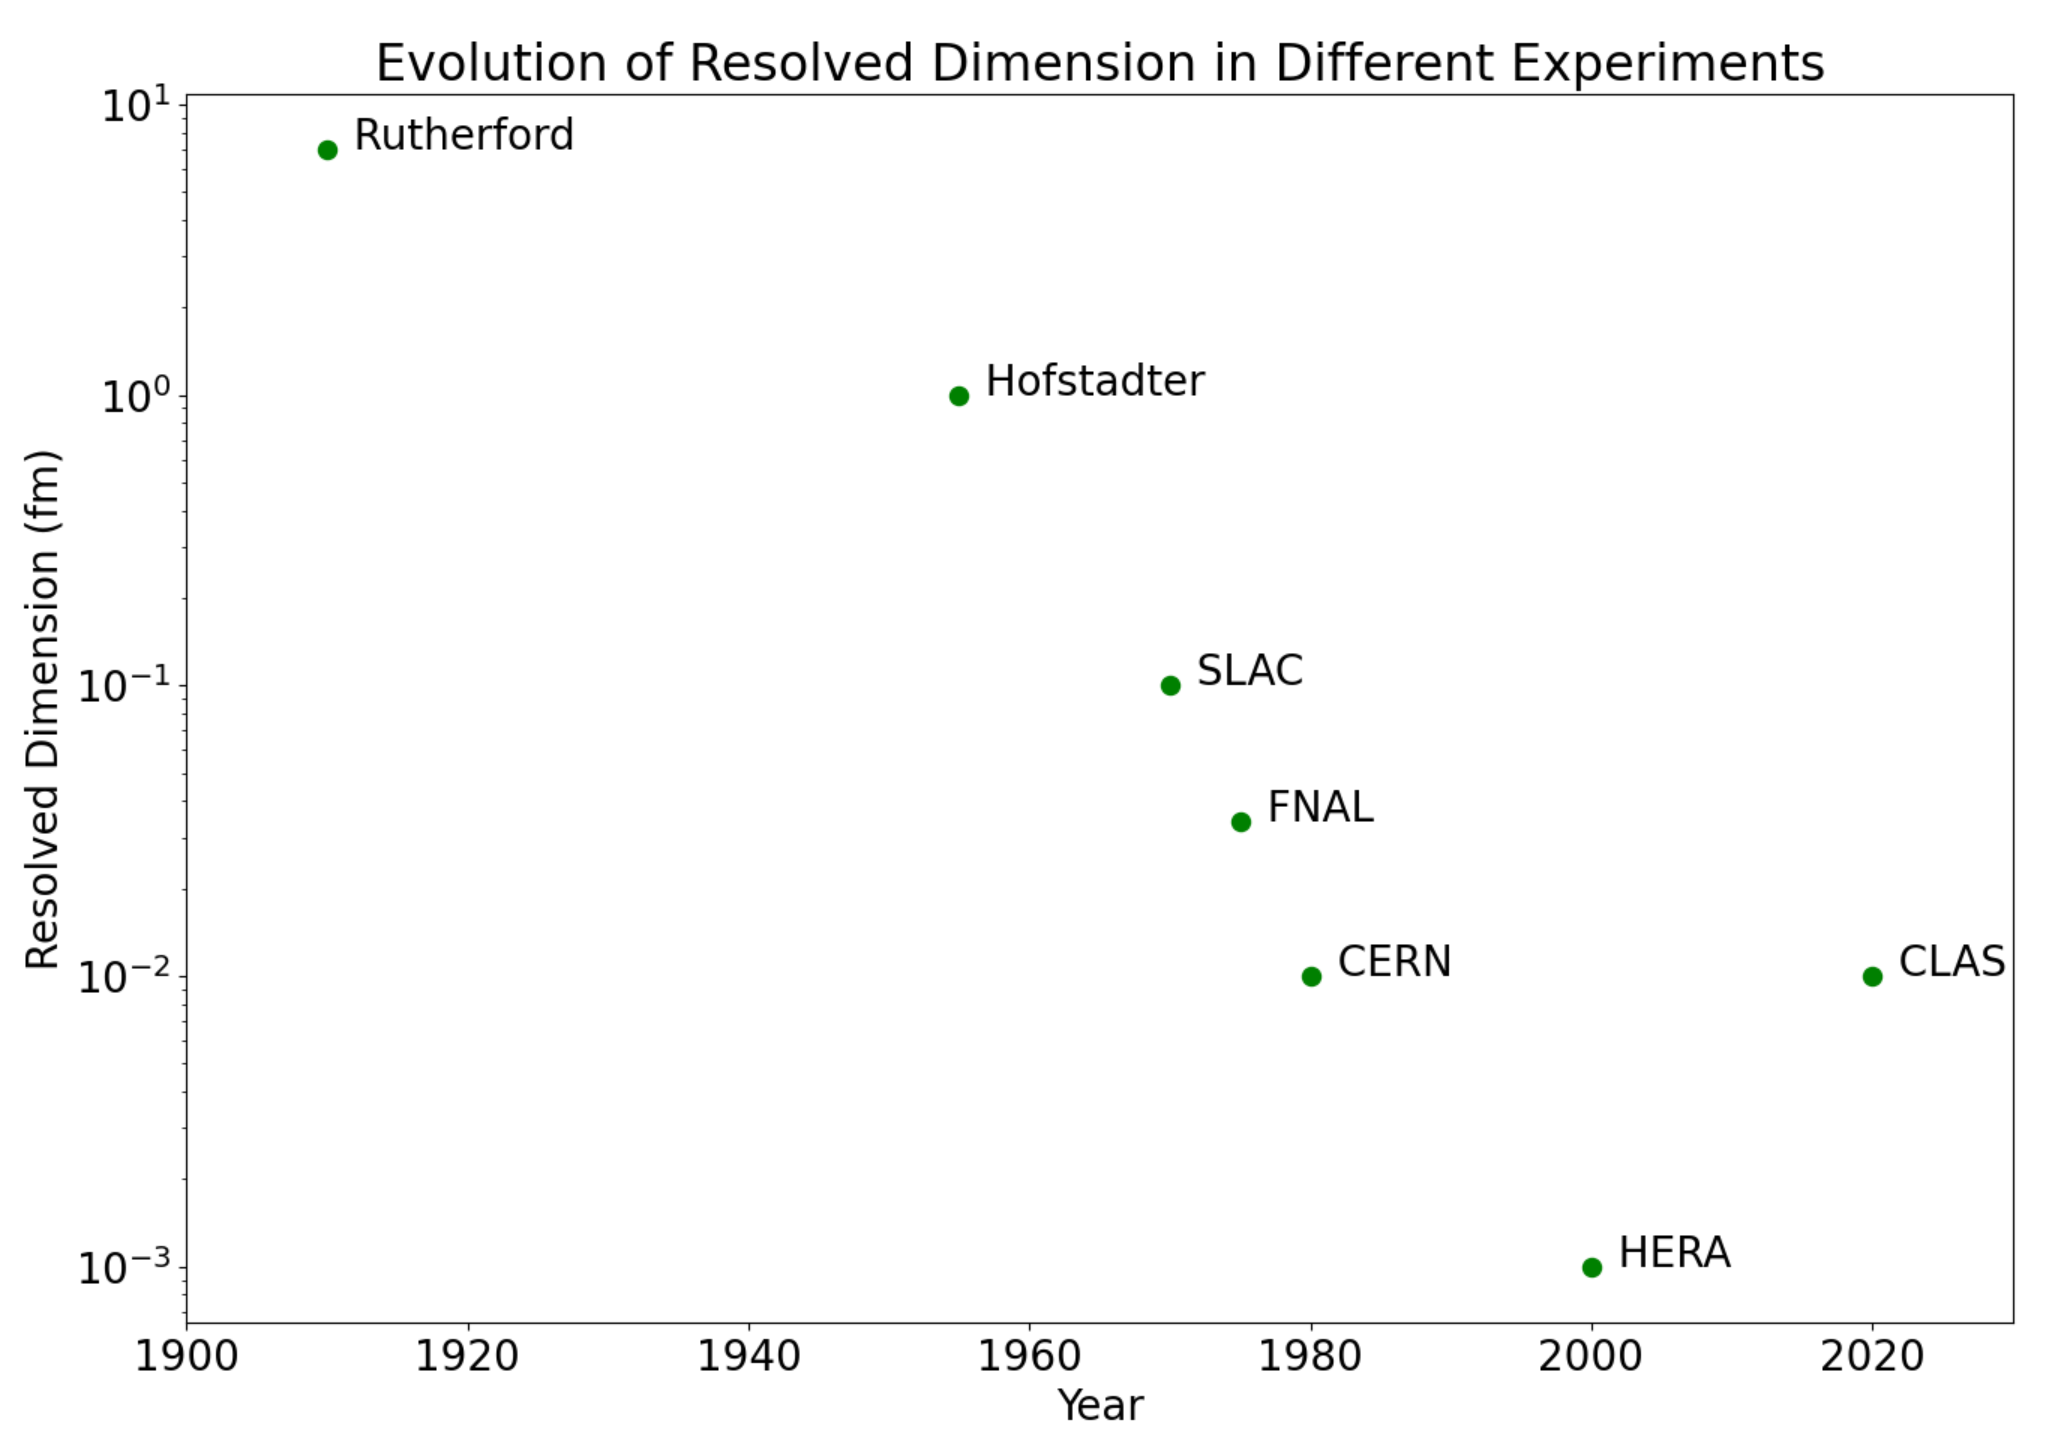
\includegraphics[width=0.9\textwidth]{Chapters/Ch1-Intro/Ch1-Sec2-GPDs-DVMP/pics/scaling.png}
    \caption{Inclusive cross section exhibits so far no extra form factor - this provides limits on SUSY, extra dimensions, quark radius, leptoquarks, etc. HERA showed quarks are pointlike down to proton radius / 100. Modified from \cite{Klein2005ResolvingHERA}}
    \label{fig:enter-label}
\end{figure}



\begin{figure}
    \centering
    \begin{tikzpicture}[
        node distance=1cm,
        box/.style={rectangle, rounded corners, draw=black, thick, minimum width=5cm, minimum height=1cm, align=center},
        bigbox/.style={rectangle, rounded corners, draw=black, thick, minimum width=10.5cm, minimum height=1cm, align=center},
        biggestbox/.style={rectangle, rounded corners, draw=black, thick, minimum width=16cm, minimum height=1cm, align=center}
    ]


    % First column
    \node[box, fill=blue!30] (c1b1) {\hyperref[sec:ch1sec2GPDs]{Underlying Physics}};
    \node[box, fill=blue!30, below=of c1b1] (c1b2)  {\hyperref[sec:clas12exp]{CLAS12 Experiment}};
    \node[box, fill=blue!30, below=of c1b2] (c1b3)  {\footnotesize Experimental Detector Signals};
    \node[bigbox, fill=orange!30, below=of c1b3, xshift=2.75cm] (c1b4)  {\hyperref[sec:decrec]{Decoding and Reconstruction}};
    \node[bigbox, fill=orange!30, below=of c1b4] (c1b5)  {\hyperref[sec:filtering]{Fiducial Filtering and File Conversion}};
    \node[box, fill=orange!30, below=of c1b5,  xshift=-2.75cm] (c1b6) {\hyperref[sec:momcorr]{Momentum Corrections}};
    \node[bigbox, fill=orange!30, below=of c1b6, xshift=2.75cm] (c1b7)  {\hyperref[sec:eventselection]{Event Selection}};
    \node[box, fill=blue!30, below=of c1b7,  xshift=-2.75cm] (c1b8) {Experimental Events};
    
    % Second column
    
    \node[box, fill=red!30, right=.5cm of c1b2] (c2b2) {\hyperref[sec:ch3gemc] {\footnotesize GEANT4 Simulation}};
    \node[box, fill=red!30, below=of c2b2] (c2b3) {\footnotesize Simulated Detector Signals};
    \node[box, fill=orange!30, right=0.5cm of c1b6] (c2b6) {\hyperref[sec:momsmear]{Momentum Smearing}};
    \node[box, fill=red!30,  right=0.5cm of c1b8] (c2b8) {Simulated Events};

    % Third column
    \node[box, fill=green!30, right=6cm of c1b1] (c3b1) {\hyperref[sec:ch3generator] {\footnotesize Computational Event Generator}};
    \node[box, fill=green!30, right=6cm of c1b8] (c3b4) {Generated Events};

    % Combined final column
    \node[biggestbox, fill=blue!30, below=of c2b8] (ccb9) {\Xsec measurement and further analysis};
    
    
    % Arrows for first column
    \draw[->] (c1b1) -- (c1b2);
    \draw[->] (c1b2) -- (c1b3);
    \draw[->] ([xshift=0cm]c1b3.south) -- ([xshift=0cm]c1b3.south |- c1b4.north);
     
    \draw[->] (c1b4) -- (c1b5);
    \draw[->] ([xshift=0cm]c1b6.north |- c1b5.south) -- ([xshift=0cm]c1b6.north);
    \draw[->] ([xshift=0cm]c1b6.south) -- ([xshift=0cm]c1b6.south |- c1b7.north);
    \draw[->] ([xshift=0cm]c1b8.north |- c1b7.south) -- ([xshift=0cm]c1b8.north);
    
    % Arrows for second column
    \draw[->] (c2b2) -- (c2b3);
    \draw[->] ([xshift=0cm]c2b3.south) -- ([xshift=0cm]c2b3.south |- c1b4.north);
    \draw[->] ([xshift=0cm]c2b6.north |- c1b5.south) -- ([xshift=0cm]c2b6.north);
    \draw[->] ([xshift=0cm]c2b6.south) -- ([xshift=0cm]c2b6.south |- c1b7.north);
    \draw[->] ([xshift=0cm]c2b8.north |- c1b7.south) -- ([xshift=0cm]c2b8.north);
    
    
    % Arrows for third column
    \draw[->] (c3b1) -- (c3b4);
    \draw[->] (c3b1) -- (c2b2);

    \draw[->] (c3b4) -- (ccb9);
    \draw[->] (c1b8) -- (ccb9);
    \draw[->] (c2b8) -- (ccb9);    
    \end{tikzpicture}
    \label{fig:ProcessFlowchart}
    \caption[Analysis Flowchart]{Analysis Processing Steps. Details on each section are hyperlinked in each box.}
\end{figure}